\documentclass[9pt,hyperref={pdfpagemode=FullScreen,urlcolor=blue},xcolor=x11names]{beamer}

\mode<presentation>
{
  \usetheme{Warsaw}
  %\usetheme{Darmstadt}
  %\usetheme{Marburg}
  \setbeamertemplate{navigation symbols}{}

  %\usecolortheme{crane}
  %\usecolortheme{rose,sidebartab}

  \usecolortheme{beaver}
  %\usecolortheme{lily,sidebartab}
  %\usecolortheme{seahorse}

  \usefonttheme{serif}

  \setbeamertemplate{footline}[page number]
  \setbeamertemplate{sidebar canvas right}[vertical shading][top=palette
  primary.bg,%,middle=white,
  bottom=palette primary.bg]
  %\setbeamertemplate{sections/subsections in toc}[section numbered,subsection numbered]

  %\setbeamertemplate{itemize subitem}[circle]

  \setbeamercovered{transparent}

  %\beamertemplatenavigationsymbolsempty

  \useinnertheme{default}
}

\usepackage[utf8]{inputenc}
\usepackage[T1]{fontenc}
\usepackage{lmodern}
\usepackage{xspace}
\usepackage{amsmath,amssymb}
\usepackage[english]{babel}
%\usepackage[latin1]{inputenc}
%\usepackage[T1]{fontenc}
\usepackage{aeguill,fourier}

% souligne, barre
\usepackage{ulem}
%\usepackage[x11names]{xcolor}

\usepackage{pgf,pgfarrows,pgfnodes,pgfautomata,pgfheaps,pgfshade}


\usepackage{wasysym}
\usepackage{fancyvrb}
%\usepackage{verbatim}
\usepackage{marvosym}

\usepackage{colortbl}

\usepackage{pdftricks}
\begin{psinputs}
\usepackage{pstricks}
\usepackage{pst-bar}
\usepackage{pstricks-add}
\end{psinputs}

\usepackage{ulem}

\usepackage{ifdraft}
\usepackage{animate}
\usepackage{multimedia}

%\usepackage{texmath}

\usepackage{tikz}
\usetikzlibrary{calc}
\usetikzlibrary{patterns}   % for hatching
\usetikzlibrary{positioning}
\usetikzlibrary{decorations.pathreplacing}
\usetikzlibrary{decorations.pathmorphing}
\usetikzlibrary{arrows, decorations.markings}
\usetikzlibrary{shapes.geometric}
\newcommand{\warningsign}{\tikz[baseline=-.75ex] \node[shape=regular polygon, regular polygon sides=3, inner sep=0pt, draw, thick] {\textbf{!}};}
\newcommand{\reddanger}{\textcolor{red}{\danger}}


% the following is from 
% http://tex.stackexchange.com/questions/4811/make-first-row-of-table-all-bold
%\usepackage{array}
%\newcolumntype{$}{>{\global\let\currentrowstyle\relax}}
%\newcolumntype{^}{>{\currentrowstyle}}
%\newcommand{\rowstyle}[1]{\gdef\currentrowstyle{#1}%
%  #1\ignorespaces
%}

\usepackage{listings}
\usepackage{minted}

\usepackage{caption}


%%%%%%%%%%%%%%%%%%%
\hypersetup{%
  pdftitle={PATC-KOKKOS-2018},%
  pdfauthor={Pierre Kestener - CEA Saclay - MDLS - http://www.maisondelasimulation.fr},
  pdfsubject={Introdcution to Kokkos},
  pdfkeywords={KOKKOS, C++, GPU},
  pdfproducer={pdflatex avec la classe BEAMER},
  bookmarksopen=false,
  urlcolor=blue
}

%%%%%%%%%%%%%%%%%%%%%%%%%%%%%%%%%%%%%%%%%%%%%%%%%%%%%%%%%%%%%%%
%%%%%%%%%%%%%%%%%%%%%%%%%%%%%%%%%%%%%%%%%%%%%%%%%%%%%%%%%%%%%%%
%%%%%%%%%%%%%%%%%%%%%%%%%%%%%%%%%%%%%%%%%%%%%%%%%%%%%%%%%%%%%%%

\title{Kokkos, Modern C++, performance portability, ...}

\author
{
  \mbox{\underline{Pierre Kestener}}\inst{1}
}

\institute[mdls sap]{%
  \inst{1}%
  CEA Saclay, DSM, Maison de la Simulation
}

\date{PATC, May 31 st - June 1st, 2018}

\pgfdeclareimage[height=0.5cm]{university-logo}{./images/Sigle-mdls}
\logo{\pgfuseimage{university-logo}}


%%%%%%%%%%%%%%%%%%%%%
\pgfdeclareimage[width=2.0cm]{sigle-cea}{./images/Sigle-mdls}
\pgfdeclareimage[width=2.0cm]{sigle-prace}{images/logo_prace}
\pgfdeclareimage[width=2.0cm]{sigle-nvidia}{images/NV_CUDA_Teaching_Center_3D.jpg}

\titlegraphic{
  % \pgfuseimage{sigle-prace}
  \hfill
  \pgfuseimage{sigle-cea}
  \hfill
  % \pgfuseimage{sigle-nvidia}
}



\begin{document}


\definecolor{green2}{rgb}{0.1,0.8,0.1} 
\definecolor{trust}{rgb}{0.71,0.14,0.07}
\definecolor{FancyPurple}{rgb}{0.5176, 0.1137, 0.2314}

\colorlet{redshaded}{red!25!bg}
\colorlet{shaded}{black!25!bg}
\colorlet{shadedshaded}{black!10!bg}
\colorlet{blackshaded}{black!40!bg}

\colorlet{darkred}{red!80!black}
\colorlet{darkblue}{blue!80!black}
\colorlet{darkgreen}{green!70!black}
\colorlet{greenshaded}{green!95!bg}
%\colorlet{coral}{Coral1!95!bg}

%red, green, blue, cyan, magenta, yellow, black, white, darkgray, gray,
%lightgray, brown, lime, olive, orange, pink, purple, teal, violet

\newcommand\myurl[1]{\textcolor{purple}{\underline{\url{#1}}}}
\newcommand\myhref[2]{\textcolor{purple}{\underline{\href{#1}{#2}}}}

\newcommand\mySmiley{\textcolor{darkgreen}{\Smiley{}}}
\newcommand\myFrowny{\textcolor{red}{\Frowny{}}}

%% Big-O notation.
\providecommand{\OO}[1]{\ensuremath{\operatorname{O}\bigl(#1\bigr)}}

% definition des couleurs pour affichage de code
\makeatletter
\def\PY@reset{\let\PY@it=\relax \let\PY@bf=\relax%
    \let\PY@ul=\relax \let\PY@tc=\relax%
    \let\PY@bc=\relax \let\PY@ff=\relax}
\def\PY@tok#1{\csname PY@tok@#1\endcsname}
\def\PY@toks#1+{\ifx\relax#1\empty\else%
    \PY@tok{#1}\expandafter\PY@toks\fi}
\def\PY@do#1{\PY@bc{\PY@tc{\PY@ul{%
    \PY@it{\PY@bf{\PY@ff{#1}}}}}}}
\def\PY#1#2{\PY@reset\PY@toks#1+\relax+\PY@do{#2}}

\def\PY@tok@gd{\def\PY@tc##1{\textcolor[rgb]{0.63,0.00,0.00}{##1}}}
\def\PY@tok@gu{\let\PY@bf=\textbf\def\PY@tc##1{\textcolor[rgb]{0.50,0.00,0.50}{##1}}}
\def\PY@tok@gt{\def\PY@tc##1{\textcolor[rgb]{0.00,0.25,0.82}{##1}}}
\def\PY@tok@gs{\let\PY@bf=\textbf}
\def\PY@tok@gr{\def\PY@tc##1{\textcolor[rgb]{1.00,0.00,0.00}{##1}}}
\def\PY@tok@cm{\let\PY@it=\textit\def\PY@tc##1{\textcolor[rgb]{0.25,0.50,0.50}{##1}}}
\def\PY@tok@vg{\def\PY@tc##1{\textcolor[rgb]{0.10,0.09,0.49}{##1}}}
\def\PY@tok@m{\def\PY@tc##1{\textcolor[rgb]{0.40,0.40,0.40}{##1}}}
\def\PY@tok@mh{\def\PY@tc##1{\textcolor[rgb]{0.40,0.40,0.40}{##1}}}
\def\PY@tok@go{\def\PY@tc##1{\textcolor[rgb]{0.50,0.50,0.50}{##1}}}
\def\PY@tok@ge{\let\PY@it=\textit}
\def\PY@tok@vc{\def\PY@tc##1{\textcolor[rgb]{0.10,0.09,0.49}{##1}}}
\def\PY@tok@il{\def\PY@tc##1{\textcolor[rgb]{0.40,0.40,0.40}{##1}}}
\def\PY@tok@cs{\let\PY@it=\textit\def\PY@tc##1{\textcolor[rgb]{0.25,0.50,0.50}{##1}}}
\def\PY@tok@cp{\def\PY@tc##1{\textcolor[rgb]{0.74,0.48,0.00}{##1}}}
\def\PY@tok@gi{\def\PY@tc##1{\textcolor[rgb]{0.00,0.63,0.00}{##1}}}
\def\PY@tok@gh{\let\PY@bf=\textbf\def\PY@tc##1{\textcolor[rgb]{0.00,0.00,0.50}{##1}}}
\def\PY@tok@ni{\let\PY@bf=\textbf\def\PY@tc##1{\textcolor[rgb]{0.60,0.60,0.60}{##1}}}
\def\PY@tok@nl{\def\PY@tc##1{\textcolor[rgb]{0.63,0.63,0.00}{##1}}}
\def\PY@tok@nn{\let\PY@bf=\textbf\def\PY@tc##1{\textcolor[rgb]{0.00,0.00,1.00}{##1}}}
\def\PY@tok@no{\def\PY@tc##1{\textcolor[rgb]{0.53,0.00,0.00}{##1}}}
\def\PY@tok@na{\def\PY@tc##1{\textcolor[rgb]{0.49,0.56,0.16}{##1}}}
\def\PY@tok@nb{\def\PY@tc##1{\textcolor[rgb]{0.00,0.50,0.00}{##1}}}
\def\PY@tok@nc{\let\PY@bf=\textbf\def\PY@tc##1{\textcolor[rgb]{0.00,0.00,1.00}{##1}}}
\def\PY@tok@nd{\def\PY@tc##1{\textcolor[rgb]{0.67,0.13,1.00}{##1}}}
\def\PY@tok@ne{\let\PY@bf=\textbf\def\PY@tc##1{\textcolor[rgb]{0.82,0.25,0.23}{##1}}}
\def\PY@tok@nf{\def\PY@tc##1{\textcolor[rgb]{0.00,0.00,1.00}{##1}}}
\def\PY@tok@si{\let\PY@bf=\textbf\def\PY@tc##1{\textcolor[rgb]{0.73,0.40,0.53}{##1}}}
\def\PY@tok@s2{\def\PY@tc##1{\textcolor[rgb]{0.73,0.13,0.13}{##1}}}
\def\PY@tok@vi{\def\PY@tc##1{\textcolor[rgb]{0.10,0.09,0.49}{##1}}}
\def\PY@tok@nt{\let\PY@bf=\textbf\def\PY@tc##1{\textcolor[rgb]{0.00,0.50,0.00}{##1}}}
\def\PY@tok@nv{\def\PY@tc##1{\textcolor[rgb]{0.10,0.09,0.49}{##1}}}
\def\PY@tok@s1{\def\PY@tc##1{\textcolor[rgb]{0.73,0.13,0.13}{##1}}}
\def\PY@tok@sh{\def\PY@tc##1{\textcolor[rgb]{0.73,0.13,0.13}{##1}}}
\def\PY@tok@sc{\def\PY@tc##1{\textcolor[rgb]{0.73,0.13,0.13}{##1}}}
\def\PY@tok@sx{\def\PY@tc##1{\textcolor[rgb]{0.00,0.50,0.00}{##1}}}
\def\PY@tok@bp{\def\PY@tc##1{\textcolor[rgb]{0.00,0.50,0.00}{##1}}}
\def\PY@tok@c1{\let\PY@it=\textit\def\PY@tc##1{\textcolor[rgb]{0.25,0.50,0.50}{##1}}}
\def\PY@tok@kc{\let\PY@bf=\textbf\def\PY@tc##1{\textcolor[rgb]{0.00,0.50,0.00}{##1}}}
\def\PY@tok@c{\let\PY@it=\textit\def\PY@tc##1{\textcolor[rgb]{0.25,0.50,0.50}{##1}}}
\def\PY@tok@mf{\def\PY@tc##1{\textcolor[rgb]{0.40,0.40,0.40}{##1}}}
\def\PY@tok@err{\def\PY@bc##1{\fcolorbox[rgb]{1.00,0.00,0.00}{1,1,1}{##1}}}
\def\PY@tok@kd{\let\PY@bf=\textbf\def\PY@tc##1{\textcolor[rgb]{0.00,0.50,0.00}{##1}}}
\def\PY@tok@ss{\def\PY@tc##1{\textcolor[rgb]{0.10,0.09,0.49}{##1}}}
\def\PY@tok@sr{\def\PY@tc##1{\textcolor[rgb]{0.73,0.40,0.53}{##1}}}
\def\PY@tok@mo{\def\PY@tc##1{\textcolor[rgb]{0.40,0.40,0.40}{##1}}}
\def\PY@tok@kn{\let\PY@bf=\textbf\def\PY@tc##1{\textcolor[rgb]{0.00,0.50,0.00}{##1}}}
\def\PY@tok@mi{\def\PY@tc##1{\textcolor[rgb]{0.40,0.40,0.40}{##1}}}
\def\PY@tok@gp{\let\PY@bf=\textbf\def\PY@tc##1{\textcolor[rgb]{0.00,0.00,0.50}{##1}}}
\def\PY@tok@o{\def\PY@tc##1{\textcolor[rgb]{0.40,0.40,0.40}{##1}}}
\def\PY@tok@kr{\let\PY@bf=\textbf\def\PY@tc##1{\textcolor[rgb]{0.00,0.50,0.00}{##1}}}
\def\PY@tok@s{\def\PY@tc##1{\textcolor[rgb]{0.73,0.13,0.13}{##1}}}
\def\PY@tok@kp{\def\PY@tc##1{\textcolor[rgb]{0.00,0.50,0.00}{##1}}}
\def\PY@tok@w{\def\PY@tc##1{\textcolor[rgb]{0.73,0.73,0.73}{##1}}}
\def\PY@tok@kt{\def\PY@tc##1{\textcolor[rgb]{0.69,0.00,0.25}{##1}}}
\def\PY@tok@ow{\let\PY@bf=\textbf\def\PY@tc##1{\textcolor[rgb]{0.67,0.13,1.00}{##1}}}
\def\PY@tok@sb{\def\PY@tc##1{\textcolor[rgb]{0.73,0.13,0.13}{##1}}}
\def\PY@tok@k{\let\PY@bf=\textbf\def\PY@tc##1{\textcolor[rgb]{0.00,0.50,0.00}{##1}}}
\def\PY@tok@se{\let\PY@bf=\textbf\def\PY@tc##1{\textcolor[rgb]{0.73,0.40,0.13}{##1}}}
\def\PY@tok@sd{\let\PY@it=\textit\def\PY@tc##1{\textcolor[rgb]{0.73,0.13,0.13}{##1}}}

\def\PYZbs{\char`\\}
\def\PYZus{\char`\_}
\def\PYZob{\char`\{}
\def\PYZcb{\char`\}}
\def\PYZca{\char`\^}
\def\PYZsh{\char`\#}
\def\PYZpc{\char`\%}
\def\PYZdl{\char`\$}
\def\PYZti{\char`\~}

\newcommand\lb{[}
\newcommand\rb{]}
\newcommand\PYbg[1]{\textcolor[rgb]{0.00,0.50,0.00}{\textbf{#1}}}
\newcommand\PYbf[1]{\textcolor[rgb]{0.73,0.40,0.53}{\textbf{#1}}}
\newcommand\PYbe[1]{\textcolor[rgb]{0.40,0.40,0.40}{#1}}
\newcommand\PYbd[1]{\textcolor[rgb]{0.73,0.13,0.13}{#1}}
\newcommand\PYbc[1]{\textcolor[rgb]{0.00,0.50,0.00}{\textbf{#1}}}
\newcommand\PYbb[1]{\textcolor[rgb]{0.40,0.40,0.40}{#1}}
\newcommand\PYba[1]{\textcolor[rgb]{0.00,0.00,0.50}{\textbf{#1}}}
\newcommand\PYaJ[1]{\textcolor[rgb]{0.73,0.13,0.13}{#1}}
\newcommand\PYaK[1]{\textcolor[rgb]{0.00,0.00,1.00}{#1}}
\newcommand\PYaH[1]{\fcolorbox[rgb]{1.00,0.00,0.00}{1,1,1}{#1}}
\newcommand\PYaI[1]{\textcolor[rgb]{0.69,0.00,0.25}{#1}}
\newcommand\PYaN[1]{\textcolor[rgb]{0.00,0.00,1.00}{\textbf{#1}}}
\newcommand\PYaO[1]{\textcolor[rgb]{0.00,0.00,0.50}{\textbf{#1}}}
\newcommand\PYaL[1]{\textcolor[rgb]{0.73,0.73,0.73}{#1}}
\newcommand\PYaM[1]{\textcolor[rgb]{0.74,0.48,0.00}{#1}}
\newcommand\PYaB[1]{\textcolor[rgb]{0.00,0.25,0.82}{#1}}
\newcommand\PYaC[1]{\textcolor[rgb]{0.67,0.13,1.00}{#1}}
\newcommand\PYaA[1]{\textcolor[rgb]{0.00,0.50,0.00}{#1}}
\newcommand\PYaF[1]{\textcolor[rgb]{1.00,0.00,0.00}{#1}}
\newcommand\PYaG[1]{\textcolor[rgb]{0.10,0.09,0.49}{#1}}
\newcommand\PYaD[1]{\textcolor[rgb]{0.25,0.50,0.50}{\textit{#1}}}
\newcommand\PYaE[1]{\textcolor[rgb]{0.63,0.00,0.00}{#1}}
\newcommand\PYaZ[1]{\textcolor[rgb]{0.00,0.50,0.00}{\textbf{#1}}}
\newcommand\PYaX[1]{\textcolor[rgb]{0.00,0.50,0.00}{#1}}
\newcommand\PYaY[1]{\textcolor[rgb]{0.73,0.13,0.13}{#1}}
\newcommand\PYaR[1]{\textcolor[rgb]{0.10,0.09,0.49}{#1}}
\newcommand\PYaS[1]{\textcolor[rgb]{0.25,0.50,0.50}{\textit{#1}}}
\newcommand\PYaP[1]{\textcolor[rgb]{0.49,0.56,0.16}{#1}}
\newcommand\PYaQ[1]{\textcolor[rgb]{0.40,0.40,0.40}{#1}}
\newcommand\PYaV[1]{\textcolor[rgb]{0.00,0.00,1.00}{\textbf{#1}}}
\newcommand\PYaW[1]{\textcolor[rgb]{0.73,0.13,0.13}{#1}}
\newcommand\PYaT[1]{\textcolor[rgb]{0.50,0.00,0.50}{\textbf{#1}}}
\newcommand\PYaU[1]{\textcolor[rgb]{0.82,0.25,0.23}{\textbf{#1}}}
\newcommand\PYaj[1]{\textcolor[rgb]{0.00,0.50,0.00}{#1}}
\newcommand\PYak[1]{\textcolor[rgb]{0.73,0.40,0.53}{#1}}
\newcommand\PYah[1]{\textcolor[rgb]{0.63,0.63,0.00}{#1}}
\newcommand\PYai[1]{\textcolor[rgb]{0.10,0.09,0.49}{#1}}
\newcommand\PYan[1]{\textcolor[rgb]{0.67,0.13,1.00}{\textbf{#1}}}
\newcommand\PYao[1]{\textcolor[rgb]{0.73,0.40,0.13}{\textbf{#1}}}
\newcommand\PYal[1]{\textcolor[rgb]{0.25,0.50,0.50}{\textit{#1}}}
\newcommand\PYam[1]{\textbf{#1}}
\newcommand\PYab[1]{\textit{#1}}
\newcommand\PYac[1]{\textcolor[rgb]{0.73,0.13,0.13}{#1}}
\newcommand\PYaa[1]{\textcolor[rgb]{0.50,0.50,0.50}{#1}}
\newcommand\PYaf[1]{\textcolor[rgb]{0.25,0.50,0.50}{\textit{#1}}}
\newcommand\PYag[1]{\textcolor[rgb]{0.40,0.40,0.40}{#1}}
\newcommand\PYad[1]{\textcolor[rgb]{0.73,0.13,0.13}{#1}}
\newcommand\PYae[1]{\textcolor[rgb]{0.40,0.40,0.40}{#1}}
\newcommand\PYaz[1]{\textcolor[rgb]{0.00,0.63,0.00}{#1}}
\newcommand\PYax[1]{\textcolor[rgb]{0.60,0.60,0.60}{\textbf{#1}}}
\newcommand\PYay[1]{\textcolor[rgb]{0.00,0.50,0.00}{\textbf{#1}}}
\newcommand\PYar[1]{\textcolor[rgb]{0.10,0.09,0.49}{#1}}
\newcommand\PYas[1]{\textcolor[rgb]{0.73,0.13,0.13}{\textit{#1}}}
\newcommand\PYap[1]{\textcolor[rgb]{0.00,0.50,0.00}{#1}}
\newcommand\PYaq[1]{\textcolor[rgb]{0.53,0.00,0.00}{#1}}
\newcommand\PYav[1]{\textcolor[rgb]{0.00,0.50,0.00}{\textbf{#1}}}
\newcommand\PYaw[1]{\textcolor[rgb]{0.40,0.40,0.40}{#1}}
\newcommand\PYat[1]{\textcolor[rgb]{0.10,0.09,0.49}{#1}}
\newcommand\PYau[1]{\textcolor[rgb]{0.40,0.40,0.40}{#1}}


% for compatibility with earlier versions
\def\PYZat{@}
\def\PYZlb{[}
\def\PYZrb{]}
\makeatother



%%%%%%%%%%%%%%%%%%%%%
% 1ere page
\begin{frame}[label=courant]
  \titlepage
\end{frame}

\begin{frame}
  \frametitle{Finite volume CFD example in Kokkos}
  
  \begin{itemize}
  \item \textbf{Use Kokkos to parallelize a finite volumes solver for CFD}: solver Euler system in 2D/3D, compressible fluid flow, hyperbolique problem
  \item Example graphics output; temporal evolution of fluid density (initial condition is a \textit{4 quadrants} Riemann problem):
  \end{itemize}
  \begin{center}
    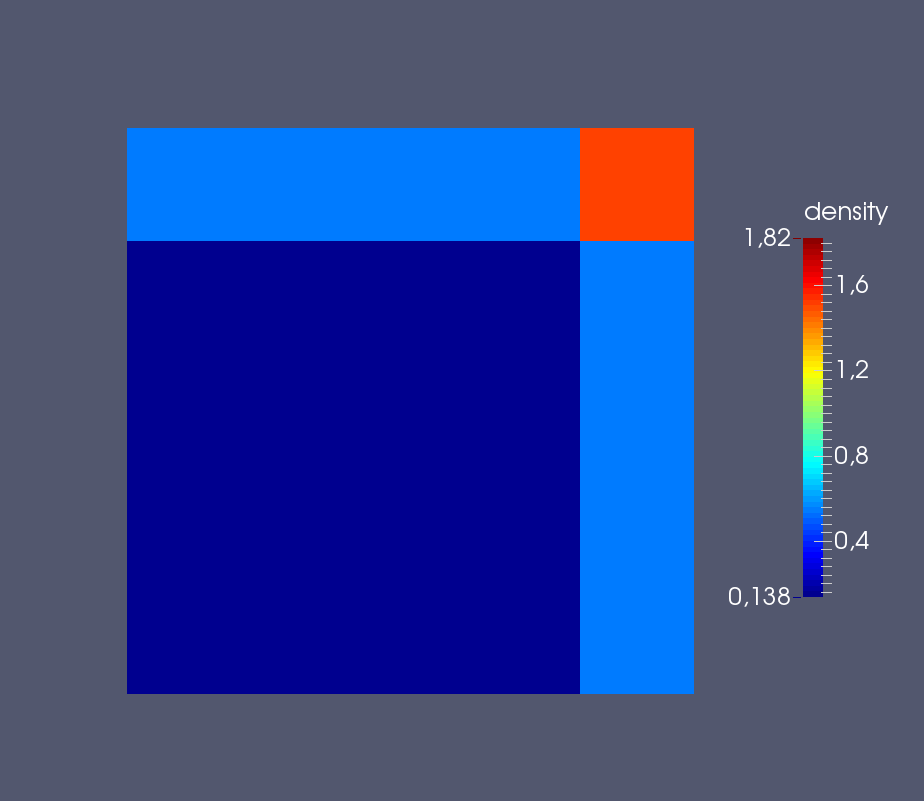
\includegraphics[height=4cm]{images/riemann/riemann_1}
    \hspace{0.1cm}
    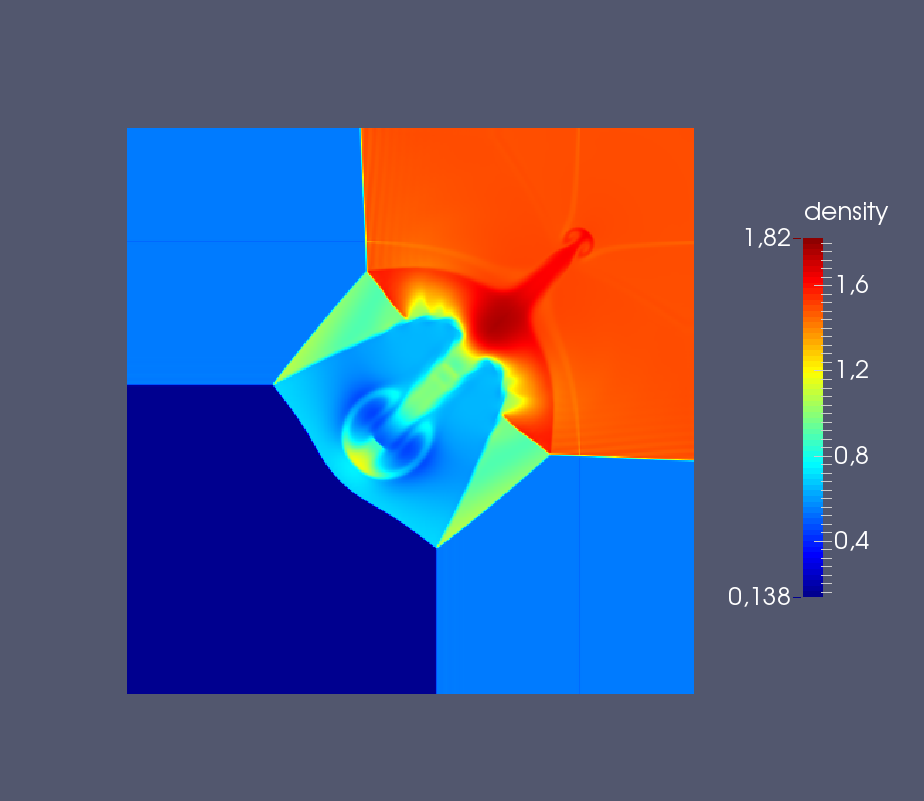
\includegraphics[height=4cm]{images/riemann/riemann_2}
  \end{center}
\end{frame}

%%%%%%%%%%%%%%%%%%%
%% Euler 3D
%%%%%%%%%%%%%%%%%%%
\begin{frame}
\frametitle{Compressible hydrodynamics : Euler equations}

\begin{itemize}
\only<1>{
\item \textbf{\textcolor{blue}{Euler equations}} (conservation of \textbf{mater}, \textbf{momentum} and \textbf{total energy})\begin{align}
  \frac{\partial\rho}{\partial t}+\mathbf{\nabla .}(\rho\mathbf{v}) & = 0\\
  \rho\frac{\partial\mathbf{v}}{\partial t}+\rho(\mathbf{v}.\mathbf{\nabla})\mathbf{v} & =  -\mathbf{\nabla} P\\
  \frac{\partial E}{\partial t} + \mathbf{\nabla}. \left[ (E+P_{tot})\mathbf{v} \right] & =  0
\end{align}}
\only<1>{
\item \textbf{\textcolor{red}{Conservative form}} : %($\partial_t \phi + \nabla \mathbf{f} =  0$) : 
$$ \mathbf{U}_t + \mathbf{F(U)}_x + \mathbf{G(U)}_y + \mathbf{H(U)}_z = \mathbf{0}$$
}
\only<1>{
\item \textcolor{darkgreen}{Conservatives variables and flux}: 
$$\mathbf{U}=\begin{bmatrix}
\rho\\
\rho u\\
\rho v\\
\rho w\\
E 
\end{bmatrix},
\mathbf{F}=\begin{bmatrix}
\rho u\\
\rho u^2+p\\
\rho uv\\
\rho uw\\
u(E+p)
\end{bmatrix},
\mathbf{G}=\begin{bmatrix}
\rho v\\
\rho vu\\
\rho v^2+p\\
\rho vw\\
v(E+p)
\end{bmatrix},
\mathbf{H}=\begin{bmatrix}
\rho w\\
\rho wu\\
\rho wv\\
\rho w^2+p\\
w(E+p)
\end{bmatrix}$$
}
\only<2>{
\item \textbf{\textcolor{red}{Conservative form}} : %($\partial_t \phi + \nabla \mathbf{f} =  0$) : 
%$$ \mathbf{U}_t + \mathbf{F(U)}_x + \mathbf{G(U)}_y + \mathbf{H(U)}_z = \mathbf{0} \Rightarrow \int_{t_n}^{t_{n+1}}\iiint_{C_{i,j,k}} \left( \mathbf{U}_t + \mathbf{F(U)}_x + \mathbf{G(U)}_y + \mathbf{H(U)}_z \right) = \mathbf{0}$$
$$ \mathbf{U}_t + \mathbf{F(U)}_x + ... = \mathbf{0} \Rightarrow \int_{t_n}^{t_{n+1}}\iiint_{C_{i,j,k}} dt \mathbf{dv} \left( \mathbf{U}_t + \mathbf{F(U)}_x + ... \right) = \mathbf{0}$$
\item After \textcolor{blue}{\textbf{time integration}} between $t_n$ and $t_{n+1}$ and over a cell volume :

  \begin{equation*} 
    \frac{\mathbf{U}_{i,j,k}^{n+1}-\mathbf{U}_{i,j,k}^{n}}{\Delta t} +
    \frac{\mathbf{F}_{i+1/2,j,k}^{n+1/2}-\mathbf{F}_{i-1/2,j,k}^{n+1/2}}{\Delta x}  + ... = 0
    %\frac{\mathbf{G}_{i,j+1/2,k}^{n+1/2}-\mathbf{G}_{i,j-1/2,k}^{n+1/2}}{\Delta y}  +
    %\frac{\mathbf{H}_{i,j,k+1/2}^{n+1/2}-\mathbf{H}_{i,j,k-1/2}^{n+1/2}}{\Delta z} = 0
  \end{equation*}
\item \textbf{$\mathbf{U}_{i,j,k}^{n}$ is a volume-averaged quantity at $t_n$}
\item \textbf{$\mathbf{F}_{i+1/2,j,k}^{n+1/2}$ is a time-averaged quantity (between $t_n$ and $t_{n+1}$, explaining index $1/2$) of the surface-average flux at $x=i+1/2$}
\item $E=\rho(\frac{1}{2}\mathbf{V}^2+e)$ Total volumic energy
\item Perfect gas law give the internal energy:
  $e=\frac{p}{\rho(\gamma-1)}$, with $\gamma=1.4$ (ex. air at $T=20^oC$)
\item {\small change to non-conservatives variables: $U \Rightarrow W$ with $^TW=[\rho, u, v, w, p]$}
}
\end{itemize}

\end{frame}

%%%%%%%%%%%%%%%%%%%%%%%%%%%%%%%%%%%%%%%%%%% 
%% Euler 3D
%%%%%%%%%%%%%%%%%%% 
\begin{frame}
  \frametitle{Godunov method - MUSCL-Hancock scheme}
%  
  \only<1>{
    \begin{minipage}{0.55\linewidth}
      \begin{itemize}
      \item $\mathbf{U}_i^{n+1} = \mathbf{U}_i^n+\frac{\Delta
          t}{\Delta x} ( \mathbf{F}_{i-\frac{1}{2}}^{n+1/2}-\mathbf{F}_{i+\frac{1}{2}}^{n+1/2} )$
      \item \textbf{How to compute/approximate flux  $\mathbf{F}_{i-\frac{1}{2}}^{n+1/2}$ ?}
      \item \textbf{\textcolor{red}{1er ordre} Godunov method :}
        % \begin{itemize}
        \item anear $x=i+1/2$, just solve a \textbf{Riemann} problem (Euler system with init conditions defined a \textcolor{red}{piecewise constants} $\mathbf{U}_{i}^{n}$ et $\mathbf{U}_{i+1}^{n}$: $\mathbf{U}^{*}_{i+1/2}=RP(\mathbf{U}_{i}^{n}, \mathbf{U}_{i+1}^{n})$
          \item then use flux $\mathbf{F}_{i+\frac{1}{2}}^{n+1/2} = F(\mathbf{U}^{*}_{i+1/2}(0))$
          \item Many type of Riemann solvers : Roe, HLL, etc ...
            % \end{itemize}
        \end{itemize}
      \end{minipage}
      % 
      \begin{minipage}{0.4\linewidth}
        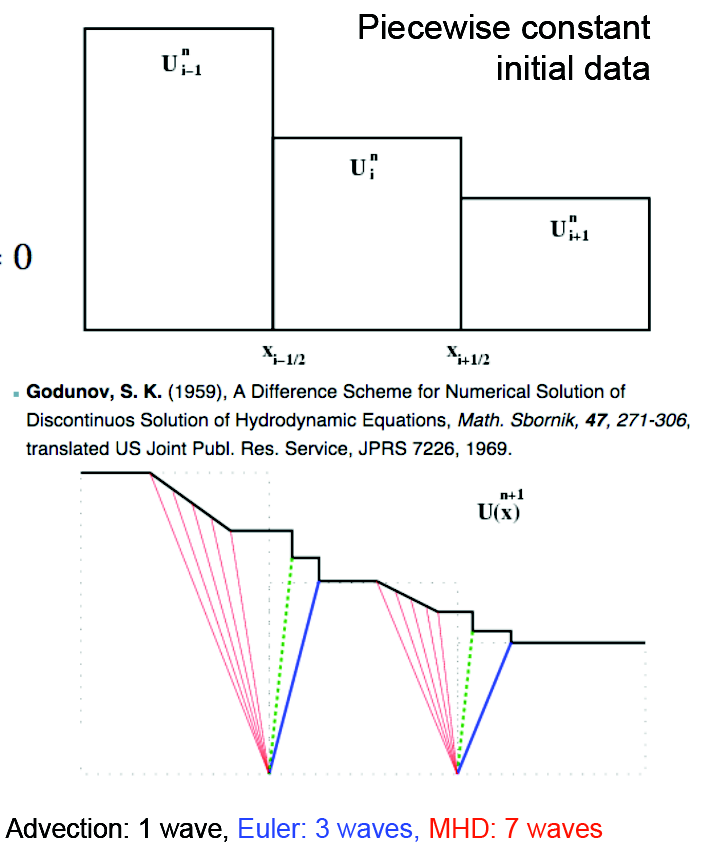
\includegraphics[height=6cm]{./images/godunov}\\
        {\tiny \textbf{Source:} R. Teyssier, 5th JETSET School, \myhref{http://irfu.cea.fr/Projets/COAST/amr_lecture1.pdf}{amr\_lecture1.pdf}\\
        book: \textit{Riemann Solvers And Numerical Methods for Fluid Dynamics: A Practical Introduction}, by E. F. Toro, Springer }
      \end{minipage}
    }
\only<2>{
\begin{minipage}{0.5\linewidth}
  \textbf{MUSCL-Hancock} (Monotone Upstream-centered Schemes for Conservation Laws) scheme implemented
\end{minipage}
\begin{minipage}{0.45\linewidth}
  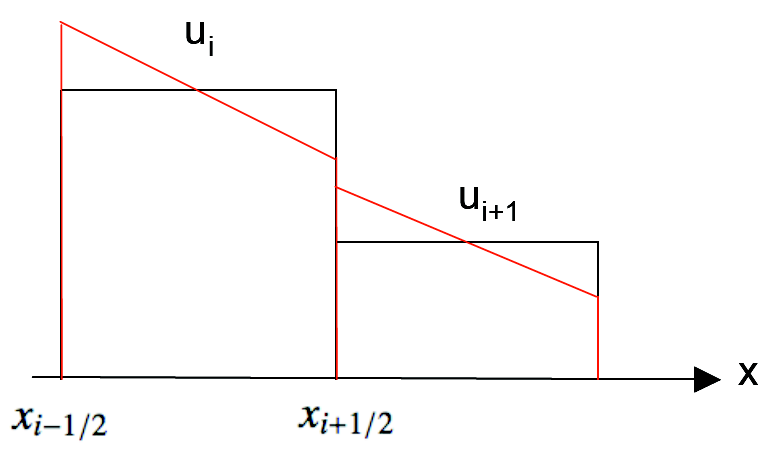
\includegraphics[height=2.8cm]{./images/godunov_2nd_ordre}\\
\end{minipage}
\begin{itemize}
\item 2nd order Godunov scheme : $\mathbf{U}_i^n$ replaced by linear picewise functions(predictor-corrector scheme).
\item MUSCL-Hancock done in 3 steps : \\
- compute slopes $\Delta_i$ (using a TVD limiter) and extrapolate $\mathbf{U_i}$ values to cell edges\\
- perform 1/2 time step integration of edge values\\
- solve Riemann problems at cell interfaces to get fluxes
$\mathbf{F_{i+\frac{1}{2}}}$, then update $\mathbf{U_i}$ at next time step
\end{itemize}
}
\end{frame}

%%%%%%%%%%%%%%%%%%%%%%%%%%%%%%%%%%%%%%%%%%%
%%%%%%%%%%%%%%%%%%%%%%%%%%%%%%%%%%%%%%%%%%%
% \begin{frame}
%   \frametitle{Sch\'ema num\'erique s\'epar\'e en direction}
% On remplace :\\
% \begin{equation*}
%   \left.
%   \begin{array}{r l}
%     \text{\textcolor{darkblue}{EDP}}  &  \quad \mathbf{U}_t + \mathbf{F(U)}_x + \mathbf{G(U)}_y + \mathbf{H(U)}_z = 0\\
%     \text{\textcolor{darkblue}{CI}}   & \quad \mathbf{U}(x,y,z,t^n)=\mathbf{U}_{i,j,k}^n\\
%     \end{array} \right\} \Rightarrow\mathbf{U}^{n+1}
% \end{equation*}
% par\\
% \begin{equation*}
%   \left.
%   \begin{array}{r l}
%     \text{\textcolor{darkblue}{EDP}}  & \quad \mathbf{U}_t + \mathbf{F(U)}_x = 0\\
%     \text{\textcolor{darkblue}{CI}}   & \quad \mathbf{U}_{i,j,k}^n \\
%   \end{array} \right\} \Rightarrow\mathbf{U}^{n+1/3}
% \end{equation*}
% %
% \begin{equation*}
%   \left.
%   \begin{array}{r l}
%     \text{\textcolor{darkblue}{EDP}}  & \quad \mathbf{U}_t + \mathbf{G(U)}_y = 0\\
%     \text{\textcolor{darkblue}{CI}}   & \quad \mathbf{U}_{i,j,k}^{n+1/3} \\
%   \end{array} \right\} \Rightarrow\mathbf{U}^{n+2/3}
% \end{equation*}
% %
% \begin{equation*}
%   \left.
%   \begin{array}{r l}
%     \text{\textcolor{darkblue}{EDP}}  & \quad \mathbf{U}_t + \mathbf{H(U)}_z = 0\\
%     \text{\textcolor{darkblue}{CI}}   & \quad \mathbf{U}_{i,j,k}^{n+2/3} \\
%   \end{array} \right\} \Rightarrow\mathbf{U}^{n+1}
% \end{equation*}
% \end{frame}


%%%%%%%%%%%%%%%%%%%%%%%%%%%%%%%%%%%%%%%%%%%
%% Structures de donn\'ees
%%%%%%%%%%%%%%%%%%%
\begin{frame}
\frametitle{Data Structures}

\begin{itemize}
\item Four 2D grids:
  \begin{itemize}
  \item 1 per conservative variable : $\rho$, $\rho v_x$, $\rho v_y$, $e$
  \item 2d space discretization
  \item limit conditions : 2 ghost cells, multiple types
    \begin{itemize}
    \item reflective
    \item absorbing
    \item periodic
    \end{itemize}
  \end{itemize}
\end{itemize}

\begin{center}
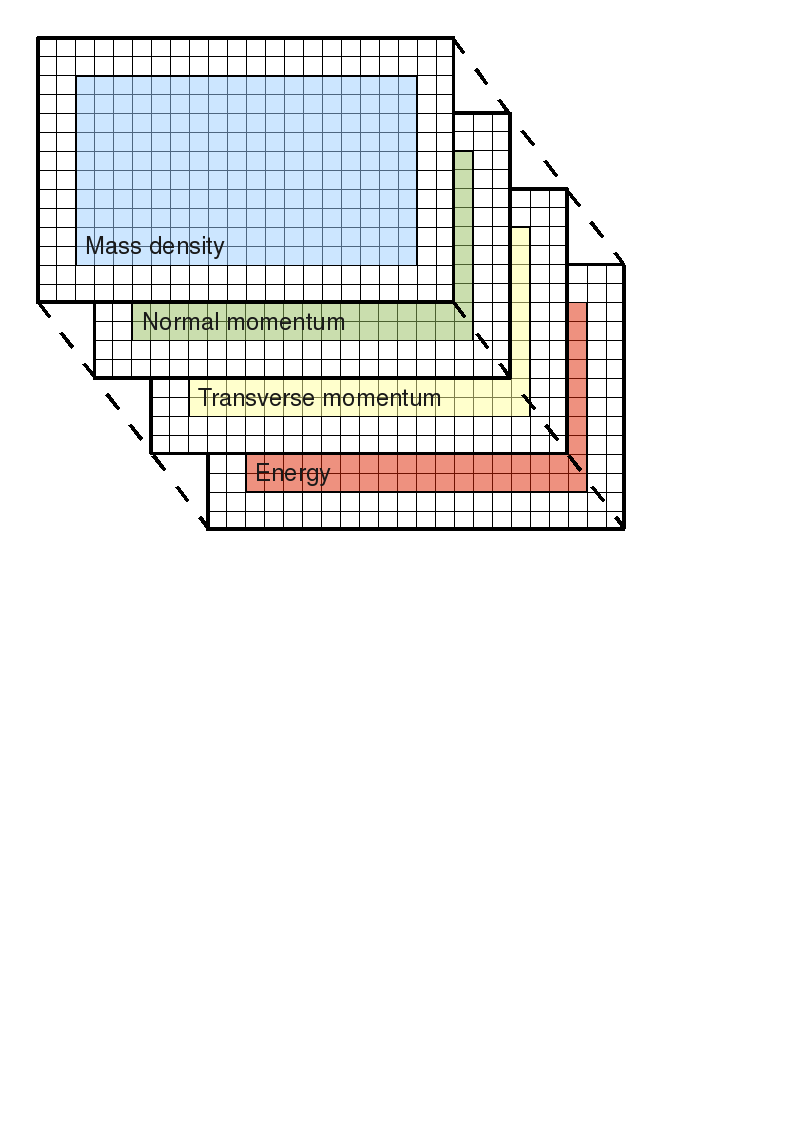
\includegraphics[height=10cm]{./images/Arrays}
\end{center}

\end{frame}

%%%%%%%%%%%%%%%%%%%%%%%%%%%%%%%%%%%%%%%%%%%
%% Simulation
%%%%%%%%%%%%%%%%%%%
\begin{frame}
\frametitle{Simulation}

\begin{itemize}
\item jet simulation
\item parameters 
\begin{itemize}
\item run parameters (total time, output rate)
\item geometric parameters (NX, NY, $\Delta x$)
\item border types
\item schmeme parameters
\item jet parameters
\end{itemize}
\end{itemize}

\begin{center}
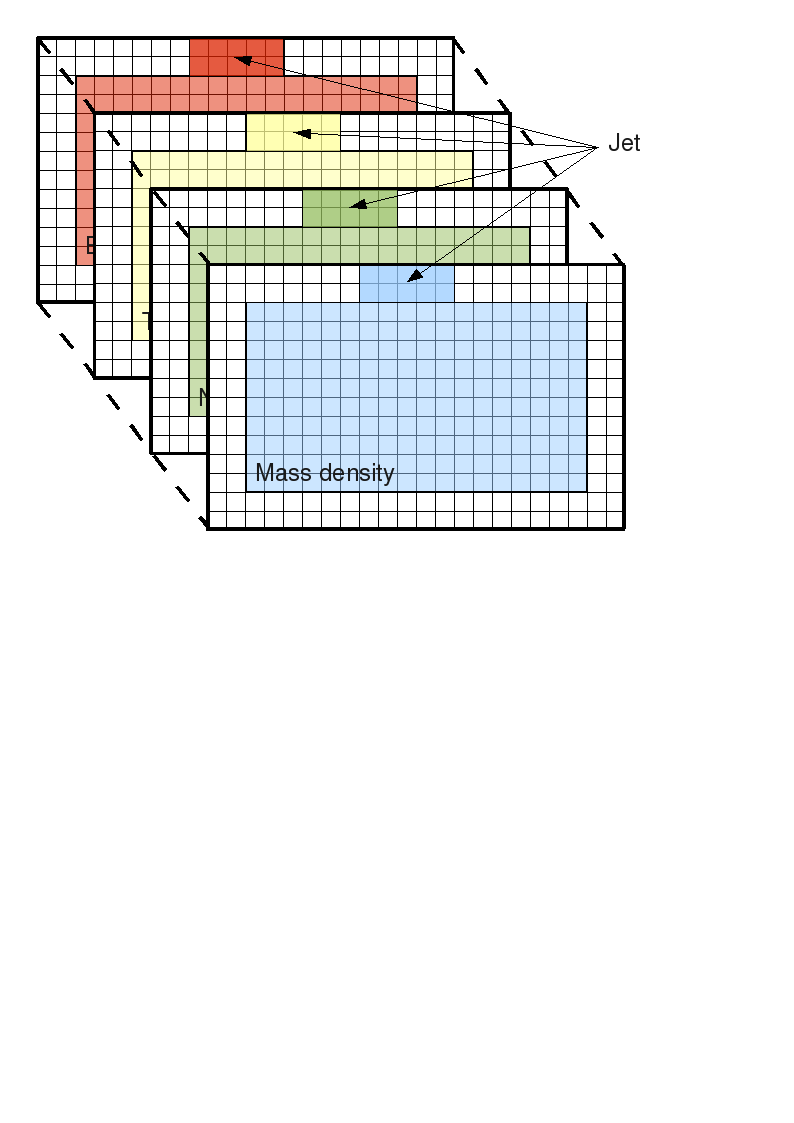
\includegraphics[height=10cm]{./images/Jet}
\end{center}

\end{frame}

%%%%%%%%%%%%%%%%%%%%%%%%%%%%%%%%%%%%%%%%%%%
%% Version s\'equentielle
%%%%%%%%%%%%%%%%%%%%%%%%%%%%%%%%%%%%%%%%%%%
\begin{frame}
\frametitle{Sequential version of \texttt{Euler2D}}

\begin{itemize}
\item How to run ?
  \texttt{./euler2d.cuda ./test.ini}
\item Quick output visualization: paraview
%\item description de l'implantation de l'algorithme de Godunov
%\item description des structures de donn\'ees
\end{itemize}

\end{frame}

%%%%%%%%%%%%%%%%%%%%%%%%%%%%%%%%%%%%%%%%%%%
%% Visualisation
%%%%%%%%%%%%%%%%%%%%%%%%%%%%%%%%%%%%%%%%%%%
\begin{frame}
\frametitle{Visualisation}

\begin{itemize}
\item File format is \myhref{http://www.vtk.org/}{VTK}: more precisely VTI (for regular cartesian grids)~\footnote{vtr format is also possible here.}; see website \myhref{http://www.cacr.caltech.edu/~slombey/asci/vtk/vtk_formats.simple.html}{vtk\_formats.simple.html} which describes VTK files format variants
\item Visualization GUI: 
  \begin{itemize}
  \item \myhref{http://www.paraview.org/}{paraview}
  \item Can also use standalone python script \texttt{plot\_data.py}
  \end{itemize}
\end{itemize}

\end{frame}

%%%%%%%%%%%%%%%%%%%%%%%%%%%%%%%%%%%%%%%%%%%
%% Reference
%%%%%%%%%%%%%%%%%%%%%%%%%%%%%%%%%%%%%%%%%%%
\begin{frame}
  \frametitle{Additional reference}
  
  \begin{itemize}
  \item See C.P. Dullemond document on CFD numerical methods: {\small \myurl{http://www.mpia-hd.mpg.de/~dullemon/lectures/fluiddynamics08/}}
  \end{itemize}

\end{frame}


\end{document}
